\documentclass{beamer}

\usepackage[bulgarian]{babel}
\usepackage{amsfonts,amsmath}
\usepackage{lmodern}
%\usepackage[notref,notcite]{showkeys}
\usepackage{graphicx}
\usepackage{wrapfig}
\usepackage{multirow}
\newcommand{\RR}{\mathbb{R}}
\newcommand{\rf}[1]{(\ref{#1})}

\usetheme{default}
\begin{document}

\title{ЧИСЛЕНО ИЗСЛЕДВАНЕ НА\\ ДВУМЕРНОТО УРАВНЕНИЕ НА БУСИНЕСК}
\author{докторант: Красимир Ангелов 
\newline \newline научен ръководител: Наталия Кольковска}

\institute[IMI -- BAS]{Институт по Математика и Информатика\\ Българска Академия на Науките, София, България,\\ e-mail: angelow@math.bas.bg}

%==================1======================================
\begin{frame}
\titlepage
\end{frame}

%---------- frame 02 ----------------
\begin{frame}
\tableofcontents 
\setbeamertemplate{table of contents shaded}[default]
\section{Въведение}
\section{Основни числени инструменти}
\section{Числени методи за двумерното стационарно уравнение на Бусинеск}
\subsection{Метод на простата итерация}
\subsection{Числени резултати}
\section{Числени методи за двумерното Парадигматично уравнение на Бусинеск (ПУБ)}
\subsection{Консервативна схема}
\subsection{Метод на Тейлор в комбинация с метод на правите}
\subsection{Числени резултати за двата метода}
\subsection{Числен тест за ПУБ при $\beta = \frac{\beta_1}{\beta_2} = 3, c=0.3$}
\section{Научни приноси}
\end{frame}

%==================3======================================
\begin{frame}
\frametitle{ Двумерното $(x,y) \in \RR^2$ Парадигматично уравнение на Бусинеск }
\begin{align}
&u_{tt} - \Delta u -\beta_1  \Delta u_{tt} +\beta_2 \Delta ^2 u +\alpha \Delta f(u)=0, \, t\in\RR^+,\label{eq1}
\\
&f(u) =  u^2 \nonumber \\  \nonumber &u(x,y,0)=u_0(x,y), \, u_t(x,y,0)=u_1(x,y)  , 
\\  &u(x,y) \rightarrow 0, \,  \Delta u(x,y) \rightarrow 0 ,  \text {при } \sqrt{x^2 + y^2} \rightarrow \infty, \label{eq11} 
\end{align}

\begin{itemize}

  \item Извеждане на {\color{red}стационарно} уравнение чрез полагането $U(x,y-ct)=u(x,y,t)$ в \rf{eq1}

{\color{red}
\begin{equation}
c^2 (E_1-\beta_1 \Delta) U_{yy} = \Delta U -\beta_2 \Delta^2 U - \Delta f(U)
\end{equation}
}%
  \item смяна на променливите:
$
x = \sqrt{\beta_1} \bar{x}, \; y = \sqrt{\beta_1} \bar{y}, \; t = \sqrt{\beta_1} \bar{t}.
$
\end{itemize}
\end{frame}


%---------- frame 03 ----------------
\begin{frame}
\frametitle{Преглед на литературата}

\begin{itemize}
  \item 2010, Christov, C.I., Kolkovska, N., Vasileva, D., On the Numerical Simulation of Un-
steady Solutions for the 2D BPE, {\it In: Numerical Methods and Applications},

  \item 2011, Chertok, A., Christov, C.I., Kurganov, A., Central-Upwind Schemes for the BPEs,
{\it Computational Science and High Performance Computing IV},

  \item 2013, Dimova M., Vasileva D., Comparison of Two Numerical Approaches to Boussinesq Paradigm Equation,  {\it Lect. Notes Comput. Sci.}, 

  \item 2013, Kolkovska, N., Angelow K., A Multicomponent Alternating Direction Method for Numerical Solving of Boussinesq Paradigm Equation, {\it In:  I. Dimov, I., Farago, I., Vulkov, L. (eds.) NAA},
    
  \item 2022, Yuyu He, Hongtao Chen, Efficient algorithm and convergence analysis of conservative SAV compact difference scheme for Boussinesq Paradigm equation, {\it Computers and Mathematics with Applications}
\end{itemize}

\end{frame}

%==================3======================================
\begin{frame}
\frametitle{Цели }
\begin{itemize}
{%\footnotesize
 \item построяване на диференчни схеми с висок ред на апроксимация (втори, четвърти и шести) върху равномерна мрежа за решаването на двумерните стационарно и хиперболично уравнения на Бусинеск;
  \item изследване на измененията в свойствата (енергията, масата, максимума и формата) на численото решение в зависимост от реда на апроксимация;
 % \item сравнение между численото решение, получено за елиптичната задача, с шести ред на апроксимация, и ``best-fit'' формулите от Пертурбационното решение на проф. Христов;
  % \item построяване на ново асимптотично гранично условие за решаването на елиптичната задача;
  %\item изследване на числените решения на хиперболичното уравнение \rf{eq1} при по-високи скорости $c$ близки до допустимия максимум $c \approx \min (\sqrt{\beta_2}/ \sqrt{\beta_1},1)$, $c < \min (\sqrt{\beta_2}/ \sqrt{\beta_1},1)$ с начално условие, получено от численото решение на елиптичната задача;
  %\item сравнение между числените резултати, получени с метода на Тейлор и други известни в литературата решения, използващи консервативни схеми с втори ред на апроксимация на вторите производни за хиперболичната задача.
  }
\end{itemize}
\end{frame}

%==================3======================================
\begin{frame}
\frametitle{Цели }
\begin{itemize}
{%\footnotesize
  %\item построяване на диференчни схеми с висок ред на апроксимация (втори, четвърти и шести) върху равномерна мрежа за решаването на двумерните стационарно и хиперболично уравнения на Бусинеск;
  %\item изследване на измененията в свойствата (енергията, масата, максимума и формата) на численото решение в зависимост от реда на апроксимация;
  %\item сравнение между численото решение, получено за елиптичната задача, с шести ред на апроксимация, и ``best-fit'' формулите от Пертурбационното решение на проф. Христов;
  %\item построяване на ново асимптотично гранично условие за решаването на елиптичната задача;
  \item изследване на числените решения на хиперболичното уравнение \rf{eq1} при по-високи скорости $c$ близки до допустимия максимум $c^2 \approx \min ({\beta_2}/ {\beta_1},1)$, $c^2 < \min ({\beta_2}/ {\beta_1},1)$ с начално условие, получено от численото решение на елиптичната задача;
  \item сравнение между числените резултати, получени с метода на Тейлор и други известни в литературата решения, използващи консервативни схеми с втори ред на апроксимация на вторите производни за хиперболичната задача.
  }
\end{itemize}
\end{frame}

%==================7.2======================================
\begin{frame}
\frametitle{Основни числени инструменти}

\begin{figure}
	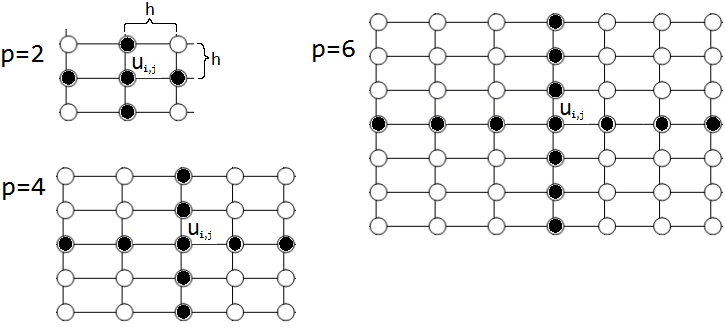
\includegraphics[width=0.99\linewidth]{FDS.png}
	\caption{Три шаблона с апроксимации $O(h^2)$, $O(h^4)$ и $O(h^6)$ за оператора на Лаплас, където $u_{i,j}:=u(x_i,y_j)$ }
	\label{fig:aproxLap}
\end{figure}

\begin{equation}\label{fdx}
\Delta_{h,p}u_{i,j} :=  \frac{1}{h^2} \sum\limits_{q=-p/2}^{p/2} d_q u(x_i+qh, y_j)+d_q u(x_i, y_j+qh), \; p=2,4,6.
\end{equation}
\end{frame}

%%==================55======================================
%
%\begin{frame}
%\frametitle{Формулировка и числено решение на двумерното стационарно уравнение на Бусинеск - Метод на простата итерация}
%\begin{itemize}
%  \item Метод на простата итерация - характеристики:
%	\begin{itemize}
%	% \item смяна на променливите: $x = \sqrt{\beta_1} \bar{x}, \quad y = \sqrt{\beta_1} \bar{y}$;
%	  \item начални данни;
%	  \item адаптивен метод за контрол на стъпката по времето;
%	  \item стоп критерий за итерационната процедура;
%	\end{itemize}
%  \item Числени резултати;
%  \item Сравнение с ``best-fit'' формулите;
%  \item Извод на ново асимптотично гранично условие.
%\end{itemize}
%\end{frame}

%==================5======================================

\begin{frame}
\frametitle{Двумерното стационарно уравнение на Бусинеск}
\framesubtitle{Метод на простата итерация [J. Choudhury, C.I. Christov, 2004]} 
 \begin{align}\label{eq3}
&c^2 \beta (E_1- \Delta) v_{{ y}{ y}} = \beta \Delta v - \Delta^2 v - \beta \Delta f(v), \quad \beta = \frac{\beta_1}{\beta_2}
\end{align}
Алгоритмични стъпки:
\begin{itemize} %две нови функции
  \item Въвеждат се: $\widehat{v}=v/{\theta} $ и $\widehat{w}=w/{\theta} $, където $v(0,0)=\theta$
\begin{align}\label{eq45}
 &- (1 - c^2 \beta) \widehat{v}_{yy} -\widehat{v}_{xx} + \beta (1-c^2) \widehat{v} - \alpha \beta \theta \widehat{v}^2 = \widehat{w}, \\
 &- \Delta \widehat{w} =  c^2 \beta \widehat{v}_{xx}.
\end{align}
%Численото решение на системата \rf{eq45} се намира чрез метода на простата итерация като изкуствено се добавят производни по времето както следва:
%\begin{itemize}
  \item Изкуствено се добавят производни по времето:
%\end{itemize}
\begin{align}\label{eq5}
\small
\begin{split}
 &\frac {\partial \widehat{v}}{\partial t} - (1 - c^2 \beta) \widehat{v}_{yy} -\widehat{v}_{xx} + \beta (1-c^2) \widehat{v} - \alpha \beta \theta \widehat{v}^2 = \widehat{w}, \\
 &\frac {\partial \widehat{w}}{\partial t} - \Delta \widehat{w} =  c^2 \beta \widehat{v}_{xx}. 
\end{split}
\end{align}
%\begin{itemize}
\item Стойността на $\theta$:
%\end{itemize}
\begin{equation}\label{eqtheta}
\small
\theta = \frac{ (1-c^2 \beta) \widehat{v}_{yy} + \widehat{v}_{xx} - \beta (1-c^2) \widehat{v} +\widehat{w}}{\alpha \beta \widehat{v}^2 } |_{x=0,y=0}.
\end{equation}
\end{itemize}
%По този начин стационарната системата от двете уравнения \rf{eq45} се заменя с преходните във времето уравнения дефинирани в \rf{eq5} с условието, че решенията $\widehat{v}$ и $\widehat{w}$ схождат линейно спрямо времето към решенията на \rf{eq45}.

\end{frame}


%%==================6======================================
%\begin{frame}
%\frametitle{Двумерното стационарно уравнение на Бусинеск}
%\framesubtitle{Метод на простата итерация} 
%Дискретизацията на последното уравнение \rf{eq5} води до следната явна схема:
%\begin{equation}\label{eq555}
%\begin{split}
%\frac {\widehat{v}^{(k+1)}-\widehat{v}^{(k)}}{\tau}- (1-c^2 \beta) \widehat{v}^{(k)}  (\Delta_{h,p,s,y})^T - \quad\quad\quad\;&\\
%-\Delta_{h,p,s,x}  \widehat{v}^{(k)}+ \beta (1-c^2 ) \widehat{v}^{(k)} - \beta \theta f(\widehat{v}^{(k)}) &= \widehat{w}^{(k)}, \\
%\frac  {\widehat{w}^{(k+1)} -\widehat{w}^{(k)}} {\tau} - \Delta_{h,p,s,x}  \widehat{w}^{(k)} - \widehat{w}^{(k)}  (\Delta_{h,p,s,y})^T &=  c^2 \beta \Delta_{h,p,s,x}  \widehat{v}^{(k)}.
%\end{split}
%\end{equation}
%
%Стойността на $\theta$ се намира използвайки следната зависимост
%\begin{equation}\label{eqtheta}
%\theta = \frac{ (1-c^2 \beta) \widehat{v}_{yy} + \widehat{v}_{xx} - \beta (1-c^2) \widehat{v} +\widehat{w}}{\alpha \beta \widehat{v}^2 } |_{x=0,y=0}.
%\end{equation}
%\end{frame}


%==================13=====================================
%\begin{frame}
%\frametitle{Ред на сходимост при Тест 1 - $\beta = 3$, $c=0.45$}
%
%\begin{table}[ht]
%\centering
%		\begin{tabular}{||c|l|ll|ll||}
%			\hline
%			\hline
%             & $h$  &  	$\Vert \bar{ E_i} \Vert_{L_2}$ 	& сход.	& $\Vert \bar{ E_i} \Vert_{L_\infty}$  		&сход.   \\
%   					\hline 
%					\hline 
%$\beta = 3$   	&0.2    										&            &            &           &   \\
%      c=0.45 	&0.1    & 0.014232  						&            & 0.016732 			&   \\
%   $O(h^2)$     &0.05   & 0.003238  						&2.14  & 0.003997					& 2.07 \\
%\hline 
%$\beta = 3$   	&0.2   &            &            &             &    \\
%      $c=0.45 $ &0.1   &   0.001758   &           &  0.002499  &   \\
%       $O(h^4)$	&0.05  &  0.000114 & 3.95    & 0.000168  & 3.90  \\
%\hline
%$\beta = 3$   	&0.2   &            &        &                  &      \\
%   $c=0.45$   	&0.1   &  0.005038 &           & 0.012462       &       \\
%     $O(h^6)$	&0.05  &  0.000094  & 5.74  &  0.000323 & 5.27         \\
%			\hline
%			\hline 
%		\end{tabular}
%		\caption{Ред на сходимост при Метода на простата итерация с апроксимации $O(h^{2})$, $O(h^{4})$ и $O(h^{6})$ за Тест  1. Грешките $\bar{ E_i}$ са пресметнати в $L_2$ и $L_\infty$ норми.}
%\label{tab:aA}
%\end{table}
%
%\end{frame}


%==================14=====================================
\begin{frame}
\frametitle{Двумерното стационарно уравнение на Бусинеск}
\framesubtitle{Ред на сходимост при $\beta = 1$, $c=0.9$}

\begin{table}[ht]
\centering
		\begin{tabular}{||c|l|ll|ll||}
			\hline
			\hline
             & $h$  &  	$\Vert \bar{ E_i} \Vert_{L_2}$ 	& сход.	& $\Vert \bar{ E_i}\Vert_{L_\infty}$  		&сход.   \\
   					\hline 					
			\hline 	
$\beta = 1$   	&0.4   &             &           &                & \\
     $c=0.9$     &0.2   &  0.043898  &             & 0.017906      &    \\
     $O(h^2)$	&0.1  & 0.009999 & 2.13       & 0.004348      & 2.04  \\
\hline 	
 $\beta = 1$   	&0.4  &            &               &               &     \\
     $c=0.9$  	&0.2   & 0.006309  &              & 0.002965      &        \\
     $O(h^4)$	&0.1  &  0.000432 &3.87        & 0.000200 &  3.89        \\
    \hline
 $\beta = 1$	&0.4   &             &        &               &        \\
   $ c=0.9$  	&0.2   &  0.000088  &        & 0.000115      &       \\
       $O(h^6)$	&0.1  &   0.000002 &5.35  & 0.000003 &   5.04       \\
	   \hline
			\hline 
		\end{tabular}
		\caption{Ред на сходимост при Метода на простата итерация с апроксимации $O(h^{2})$, $O(h^{4})$ и $O(h^{6})$ и Тест 2. Грешките $\bar{ E_i}$ са пресметнати в $L_2$ и $L_\infty$ норми.}
\label{tab:aB}
\end{table}

\end{frame}

%==================16=====================================
\begin{frame}
\frametitle{Двумерното стационарно уравнение на Бусинеск}
\framesubtitle{Форма на решението}
\begin{figure}[ht]
	\begin{minipage}[b]{0.45\linewidth}
		\raggedleft
		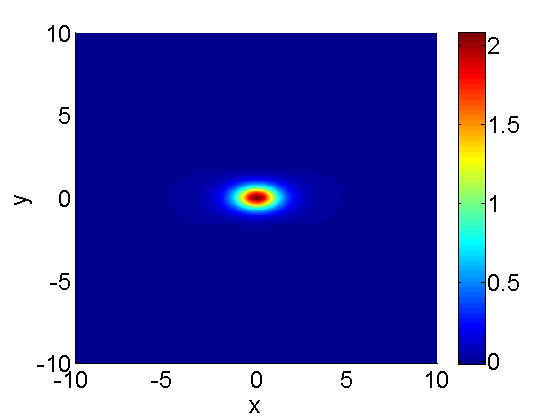
\includegraphics[width=\linewidth]{../Thesis/SolutionView/ChristovIC_30_bt3_c045_topview.png}
	\end{minipage}
	\begin{minipage}[b]{0.45\linewidth}
		\raggedright
		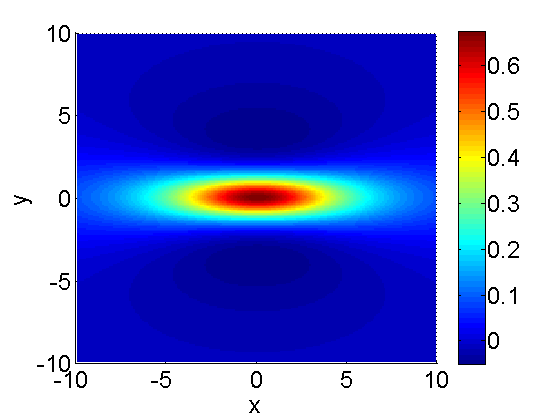
\includegraphics[width=\linewidth]{../Thesis/SolutionView/ChristovIC_128_bt1_c090_topview.png}
	\end{minipage}
	\begin{minipage}[b]{0.45\linewidth}
		 \raggedleft
		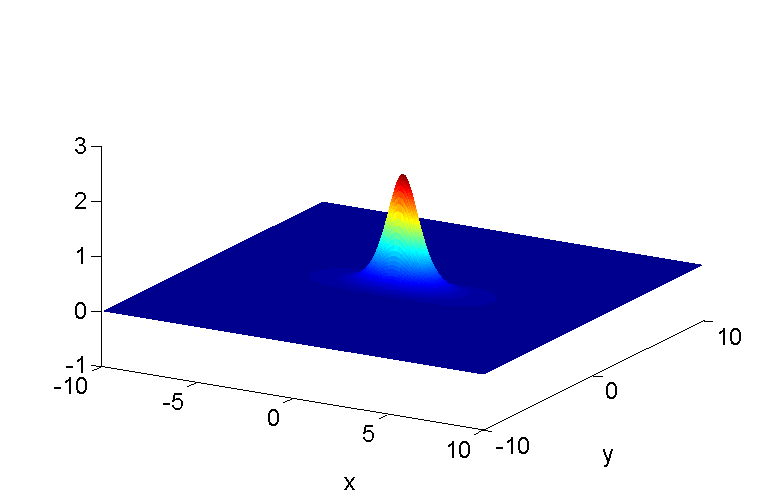
\includegraphics[width=\linewidth]{../Thesis/SolutionView/ChristovIC_30_bt3_c045_prpview.png}		
		\centerline{$\beta = 3$, $c = 0.45$ }
	\end{minipage}
	\begin{minipage}[b]{0.45\linewidth}
		 \raggedright
		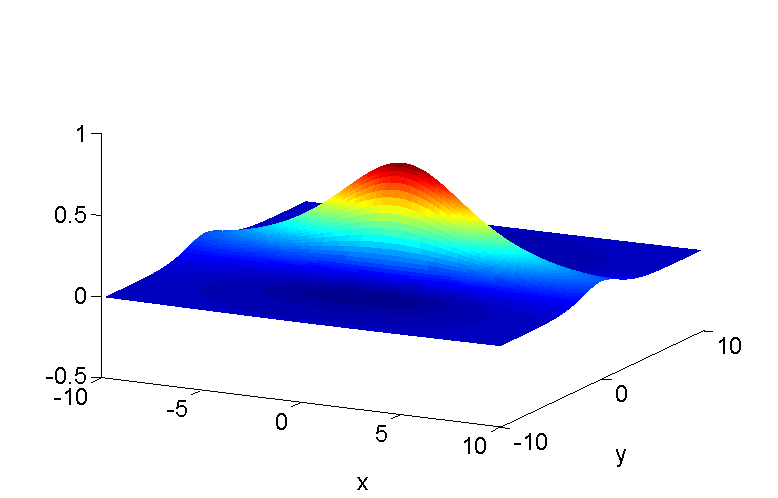
\includegraphics[width=\linewidth]{../Thesis/SolutionView/ChristovIC_128_bt1_c090_prpview.png}
		\centerline{$\beta = 1$, $c = 0.9$}
	\end{minipage}
	\caption{2D и 3D профили на численото решение $\widehat v$.}
	\label{fig:solutions}
\end{figure}

\end{frame}

%==================5======================================

%---------- frame 08 ----------------
\begin{frame}
\frametitle{Двумерното Парадигматично уравнение на Бусинеск}
\framesubtitle{Масата и енергията за непрекъснатата задача }
\begin{itemize}
\item {\footnotesize Christov C., An energy-consistent dispersive shallow-water model.}
\end{itemize}
Масата:
\begin{equation}\label{intM}
M(u(x,y,t))=\int_{\RR^2} u(x,y,t)dx dy = const.
\end{equation}

Енергията:
\begin{align}\label{ex-en}
E(u(x,y,t)) = &\int_{R^2} u_t \left(((-\Delta)^{-1}+E)u_t\right) dxdy+
\beta \int_{R^2} u^2 dxdy \nonumber\\
-& \int_{R^2}u \left(\Delta u\right) dxdy
-\frac{2 \alpha \beta}{3} \int_{R^2} u^3 dxdy =const.
\end{align}

\end{frame}

%---------------------------- frame 15 --------------------------------------
\begin{frame}
\frametitle{Двумерното Парадигматично уравнение на Бусинеск}
\framesubtitle{Консервативна схема}
\begin{itemize}
\footnotesize
\item Kolkovksa, N., Dimova, M., {\it Cent. Eur. J. Math.}, 2012
\end{itemize}

\begin{align}\label{consFDS}
\beta (E_1-\Delta_{h,2})&\frac{ u^{(k+1)}_{i, j} - 2u^{(k)}_{i,j} + u^{(k-1)}_{i,j} }{\tau^2} =  \nonumber \\
&=(\Delta_{h,2} - \Delta_{h,2}^2)u^{(k)}_{i,j} + \Delta_{h,2}(g(u^{(k)}_{i,j})),
\end{align}
където:
\begin{align}
g(u^{(k)}_{i,j})=& -\frac{\alpha \beta} { 3 } \left( (u^{(k+1)}_{i,j})^2 + (u^{(k-1)}_{i,j})(u^{(k+1)}_{i,j}) + (u^{(k-1)}_{i,j})^2 \right) + \nonumber\\
+&\frac{ (\beta - 1 )}{ 2 }\left( u^{(k+1)}_{i,j} + u^{(k-1)}_{i,j} \right).
\end{align}
\end{frame}

%------------------------- frame 14 -----------------------------------------

\begin{frame}
\frametitle{Двумерното Парадигматично уравнение на Бусинеск}
\framesubtitle{Метод на Тейлор и метод на правите за ПУБ}

Дискретизация по пространството води до следната система от ОДУ:
\begin{equation}\label{DiscreteEq}
\beta (I-\Delta_{h,p}) \frac{\partial^2 u}{\partial t^2}(x_i, y_j, t)=
 (\Delta_{h,p} - \Delta_{h,p}^2) u_{i, j}(t) + \Delta_{h,p} ( ( u_{i, j}(t) )^2 )
\end{equation}
за $i = 0..N_1$ и $j=0..N_2$, и $\beta = \frac{\beta_1}{\beta_2}$. За всяко ОДУ от системата е направено развитие в ред на Тейлор:
\begin{align} \label{TSe}
\small
u(x_i, y_j, {\small t+\tau}%
) = u(x_i, y_j, t) + \tau \frac{ \partial u }{ \partial t }(x_i, y_j, t)  +  \frac{\tau^2}{2} \frac{ \partial^2 u }{ \partial t^2 }(x_i, y_j, t)  + ... 
\nonumber
\\
\frac{ \tau^p }{ p! } \frac{ \partial^p u }{ \partial t^p }(x_i, y_j, t) + O(\tau^{p+1})
\end{align}

Така се получават следните апроксимации
\begin{description}
 \item[$p=2,4,6$] $O(|h|^p + \tau^p)$
\end{description}

\end{frame}

%---------------------------- frame 15 --------------------------------------


\begin{frame}
\frametitle{Двумерното Парадигматично уравнение на Бусинеск}
\framesubtitle{Числени резултати - параметри}

Дисперсионен параметър $\beta= \frac{\beta_1}{\beta_2}$, скорост $c$, време $T$ и големина на областта
\begin{description}
 \item[Тест 1] $\beta = 3$, $c = 0.45$, $\Omega = [-30, 30] \times [-27, 27]$, $T = 10$
 \item[Тест 2] $\beta = 1$, $c = 0.9$, $\Omega = [-128, 128] \times [-58, 58]$, $T = 10$
\end{description}

Ред на апроксимация $p$
\begin{enumerate}
  \item Консервативна схема с $O(|h|^2 + \tau^2)$
  \item метод на Тейлор с $O(|h|^p + \tau^p)$ и $p = 2, 4, 6$
\end{enumerate}

Тест 1 and Тест 2 използват 
\begin{itemize} 
\item нулево гранично условие - по границата на областта се използват несиметрични крайни разлики,
\item начално условие от численото решение на стационарното уравнение на Бусинеск.
\end{itemize}
\end{frame}

%---------------------------- frame 17 --------------------------------------

\begin{frame}
\frametitle{Двумерното Парадигматично уравнение на Бусинеск}
\framesubtitle{Сходимост}

\begin{table}[ht]
\centering
\resizebox{0.8\linewidth}{!}{%
		\begin{tabular}{||c|l|ll|ll||}
			\hline
			\hline
      \multirow{2  }{*}{ $T = 10$ }        & \multirow{2  }{*}{$h$, $\tau$}  & \multirow{2  }{*}{грешки $\Vert E_i \Vert_{L_2}$ } &ред на& \multirow{2  }{*}{грешки $\Vert E_i \Vert_{L_\infty}$}  &ред на  \\
	         &                    &                               & сход   &                                        & сход. \\
\hline 
\hline 
  $\beta=3$               &0.2, 0.1      &              	&           &                	&      \\
   c=0.45                   &0.1, 0.05    &0.968044  	&           &1.034208   &       \\
 $O(h^2 + \tau^ 2)$ 	&0.05, 0.025	& 0.340955 	& 1.51    &0.351518  	&  1.56      \\
\hline 
  $\beta=3$               &0.2, 0.1      &              	&          	&                 &      \\
   c=0.45                   &0.1, 0.05    &0.191389 	&          	&0.194056   	&       \\
$O(h^4+ \tau^4)$	&0.05, 0.025	&0.013036 	& 3.88   	&0.013664   	& 3.83       \\
\hline 
  $\beta=3$               &0.2, 0.01    &                	&          	&                 &      \\
     c=0.45                 &0.1, 0.05    &0.032671 	&          	& 0.033625  	&       \\
  $O(h^6+ \tau^6)$ 	&0.05, 0.025	&0.000599 	&5.78    	& 0.000635  	& 5.73       \\
\hline
\hline 
       $\beta=1$        	&0.4, 0.2      &             	&            &           &   \\
           c=0.9    		&0.2, 0.1      &  0.148014 	&            &0.058905 &   \\
  $O(h^2+ \tau^2)$  	&0.1, 0.05   	& 0.030690  	&2.27  	 &0.014185   & 2.05 \\
\hline
      $\beta=1$           &0.4, 0.2    	&            	&               &             &    \\
       c=0.9                 &0.2, 0.1     & 0.028869   &        &  0.013791   &   \\
 $O(h^4+ \tau^4)$ 	&0.1, 0.05   	&0.001860 	& 3.96  & 0.000996  & 3.80  \\
\hline
  $\beta=1$     		&0.4, 0.2   	&            	&          	&                  &      \\
      c=0.9                  &0.2, 0.1   	&0.006732 	&            & 0.003334      &       \\
 $O(h^6+ \tau^6)$ 	&0.1, 0.05 	& 0.000249 	& 4.75 	& 0.000068  & 5.61        \\
\hline
\hline 
		\end{tabular}
		}%
		\caption{Скорост на сходимост на численото решение при метода на Тейлор с грешки $O(h^{2} + \tau^2 )$, $O(h^{4} + \tau^4 )$ и $O(h^{6} + \tau^6 )$. }
\label{table:A}
\end{table}

\end{frame}
%------------------------------ frame 19 ------------------------------------

\begin{frame}
\frametitle{Двумерното Парадигматично уравнение на Бусинеск}
\framesubtitle{Дискретна енергия - сравнение между метода на Тейлор и Консервативната схема}

\begin{center}\vspace{0.4cm}
	\begin{minipage}[b]{0.49\linewidth}
		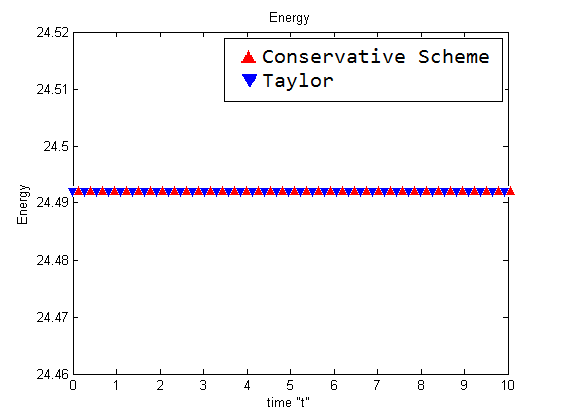
\includegraphics[width=\linewidth]{Energy_bt3_c045_h005.png}
	\end{minipage}	
	\begin{minipage}[b]{0.49\linewidth}
		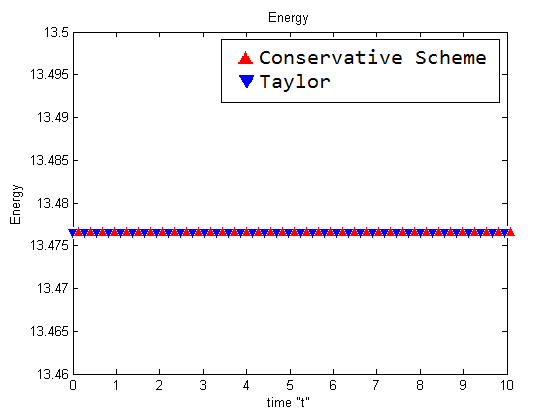
\includegraphics[width=\linewidth]{Energy_bt1_c090_h010.png}
		
	\end{minipage}
\end{center}
Дискретната енергия като функция на времето до $T = 10$ при Тест 1 (ляво) и Тест 2 (дясно) и апроксимация $O(|h|^2 + \tau^2)$.
\end{frame}

%---------------------------------- frame 18 --------------------------------

\begin{frame}
\frametitle{Двумерното Парадигматично уравнение на Бусинеск}
\framesubtitle{Дискретна маса - сравнение между метода на Тейлор и Консервативната схема}

\begin{figure}[ht]\vspace{0.4cm}
	\begin{minipage}[b]{0.49\linewidth}
		 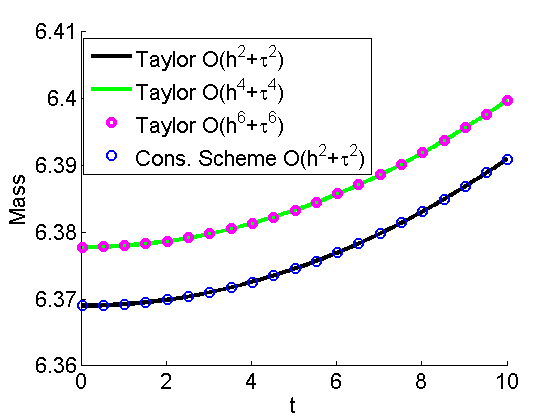
\includegraphics[width=\linewidth]{Mass_bt3_c045_h005_Oh2_Oh4_Oh6.png}
	\end{minipage}	
	\begin{minipage}[b]{0.49\linewidth}
		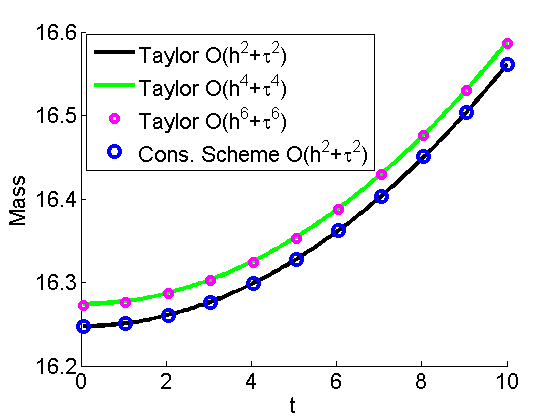
\includegraphics[width=\linewidth]{Mass_bt1_c090_h010_Oh2_Oh4_Oh6.png}	
	\end{minipage}
\caption{Дискретната маса като функция на времето до $T = 10$ при Тест 1 (ляво) и Тест 2 (дясно).}
\label{Test1En}
\end{figure}

\end{frame}

%---------------------------------- frame 20 --------------------------------

\begin{frame}
\frametitle{Двумерното Парадигматично уравнение на Бусинеск}
\framesubtitle{Дискретна маса при по-големи области}
\begin{center}\vspace{0.4cm}
	\begin{minipage}[b]{0.49\linewidth}
		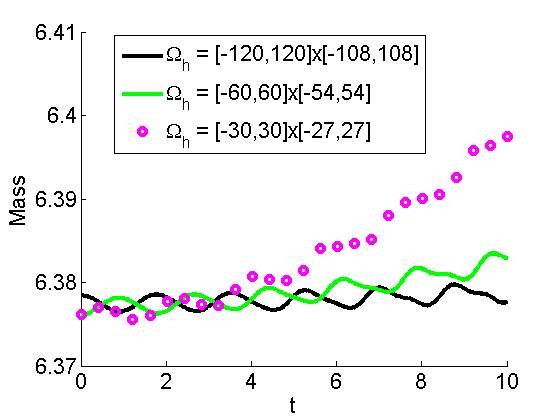
\includegraphics[width=\linewidth]{MassTaylor_120_60_30_ZB1_bt3_c045_h020_O(h^6).png}
	\end{minipage}	
	\begin{minipage}[b]{0.49\linewidth}
		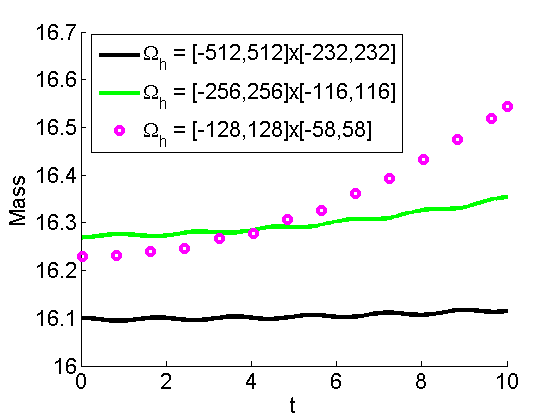
\includegraphics[width=\linewidth]{MassTaylor_512_256_128_ZB1_bt1_c090_h040_O(h^6).png}
		
	\end{minipage}
\end{center}
Масата при апроксимация $O(|h|^6 + \tau^6)$ и време $T = 10$ върху три вложени области. Левия панел е при $\beta=3$, $c = 0.45$, а десния при $\beta=1$, $c = 0.9$.
\end{frame}


%---------------------------------- frame 20 --------------------------------

\begin{frame}
\frametitle{Двумерното Парадигматично уравнение на Бусинеск}
\framesubtitle{Форма - сравнение между метода на Тейлор и Консервативната схема}
\begin{table}
\centering
\small
\resizebox{1\linewidth}{!}{%
		\begin{tabular}{||c|l|l|l|l||}
			\hline
			\hline
      $p=2$         &$h$, $\tau$  &   $||uC - uT||_{L_2}$     &  $||uC - uT||_{L_\infty}$ & $||uC||_{L_\infty}$ \\
   			\hline 
					\hline 
  $\beta=3$                  &0.2, 0.1         &  1.803e-01       &  2.037e-01& 1.316884     \\
   c=0.45                      &0.1, 0.05       &  8.195e-02       & 8.355e-02 	&  1.835198     \\
     $O(h^2 + \tau^ 2)$ &0.05, 0.025   & 2.480e-02        &2.522e-02  	&   2.004938   \\
			\hline 
			\hline 
       $\beta=1$          &0.4, 0.2        & 5.629e-02      & 2.554e-02 & 0.660152   \\
                  c=0.9      &0.2, 0.1        & 1.077e-02      & 3.862e-03  & 0.672095   \\
  $O(h^2+ \tau^2)$ &0.1, 0.05         & 2.606e-03     & 9.652e-04 & 0.671322   \\
			\hline
	   \hline
			\hline 
		\end{tabular}
		}
		\caption{Разлики $uC - uT$ между двата класа от решения получени от Консервативната схема и метода на Тейлор за време $t=10$ и апроксимация $O(|h|^2 + \tau^2)$. Разликите са измерени в $L_2$ и $L_\infty$ норми.}
\label{tableF}
\end{table}
% $\tau = h/100$,
\end{frame}


%---------------------------------- frame 24 --------------------------------

\begin{frame}
\frametitle{Двумерното Парадигматично уравнение на Бусинеск}
\framesubtitle{Числен Тест по метода на Тейлор при $\beta = 3, c=0.3$}

Дисперсионен параметър $\beta= \frac{\beta_1}{\beta_2}$, скорост $c$, време $T$ и големина на областта
\begin{description}
 \item[Тест 3] $\beta = 3$, $c = 0.3$, $\Omega = [-50, 50] \times [-50, 50]$, $T = 10$
\end{description}

Метод на Тейлор с 
\begin{enumerate}
  \item $O(|h|^p + \tau^p)$, $p = 4, 6$
  \item $(h, \tau)=(0.1, 0.05), (0.2, 0.1), (0.4, 0.2)$
\end{enumerate}

Тест 3 използва 
\begin{itemize} 
\item нулево гранично условие - по границата на областта се използват несиметрични крайни разлики,
\item начално условие от численото решение на стационарното уравнение на Бусинеск.
\end{itemize}
\end{frame}


%---------------------------------- frame 27 --------------------------------
\begin{frame}
\frametitle{Двумерното Парадигматично уравнение на Бусинеск}
\framesubtitle{Форма на решението в зависимост от дискретните стъпки и реда на апроксимация}

\begin{table}[ht]
\centering
\small
		\begin{tabular}{||c|l|l|l||}
			\hline
			\hline
  $p=4,6$   &  $h, \tau$ &  $||u^{(0)} - u^{(N_t)}||_{L_2}$  & $||u^{(0)} - u^{(N_t)}||_{L_\infty}$   \\
   		      \hline 
			\hline
           				& $0.4, 0.2$   &  3.020072 & 2.571611     \\
			\hline 
  $O(|h|^4+\tau^4)$ & $0.2, 0.1$   & 0.365473 & 0.371433      \\
			\hline 
           				& $0.1, 0.05$ & 0.025631 & 0.026517      \\
	   \hline
          \hline
           				& $0.4, 0.2$   & 1.939208 & 1.673675      \\
			\hline
  $O(|h|^6+\tau^6)$ & $0.2, 0.1$   & 0.037638 & 0.038985      \\
    \hline
           				& $0.1, 0.05$  & 0.000655 & 0.000679       \\
	   \hline
		\hline 
		\end{tabular}
		\caption{Разликата $||u^{(0)} - u^{(N_t)}||_\kappa$ в $L_2$ и $L_\infty$ норми между числените решения в началото при $t=0$ и в края при $t=10$. За резултатите в таблицата е използван метода на Тейлор с четвърти и шести порядък на апроксимация. }
\label{tableK}
\end{table}

\end{frame}

%---------------------------------- frame 28 --------------------------------
\begin{frame}
\frametitle{Двумерното Парадигматично уравнение на Бусинеск}
\framesubtitle{Максимума на решението в зависимост от дискретните стъпки и реда на апроксимация}
\begin{figure}
	%\centering
	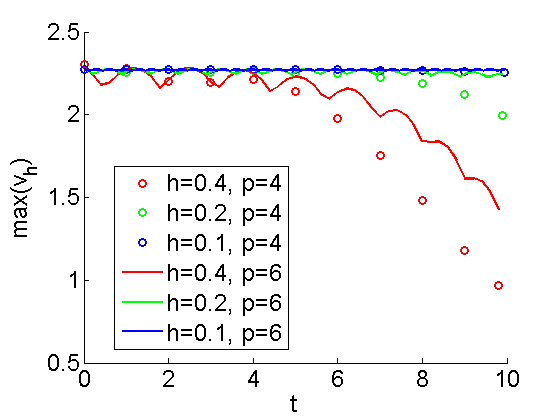
\includegraphics[width=0.65\linewidth]{Maximum_TaylorZeroBnd_50x50_bt3_c030.png}
\caption{Развитие на максимума на решението в интервала $[0, 10]$}

\end{figure}

\end{frame}
%------------------------------------------------------------------

%==================30=====================================
\begin{frame}
\frametitle{Научни приноси}

\begin{itemize}
{\small
  \item Разработили сме числени методи с четвърти и шести ред на апроксимация за стационарното и Парадигматичното уравнения на Бусинеск;
  \item Изследвали сме подробно асимптотиката на всеки един от членовете в елиптичното уравнение и сме изведели ново асимптотично гранично условие; 
  \item Числените експерименти демонстрират, че формата и максимума се запазват по-добре, когато се използват по-ситни дискретни стъпки и по-висок ред на апроксимация за фиксиран интервал от време $T$;
  \item Mетодът на Тейлор запазва енергията и масата толкова добре колкото и Консервативната схема при разгледаните числени тестове;
 %\item Направено е подробно сравнение между ``best-fit'' формулите и решението от елиптичната задача при $O(h^6)$.
%    \item Показали сме, че началното условие, получено чрез итерационен метод с висок ред на апроксимация за решаване на стационарното уравнение, превъзхожда ``best-fit'' апроксимационните формули, когато се изследва солитонният характер на вълната в ПУБ, защото нейните форма и максимум се запазват за по-дълъг период от време;
}
\end{itemize}

\end{frame}

%---------- frame 05 ----------------

\begin{frame}
\frametitle{Публикации}

Резултатите от численото решение на двумерните стационарно и хиперболични уравнения на Бусинеск са
публикувани в
\begin{itemize}
  \item N. Kolkovska, K. Angelow, Numerical computation of the critical energy constant for two dimensional Boussinesq equations, {\it Appl. of Mathematics in Technical and Natural Sciences}, 1684 (2015), SJR
  \item K. Angelow, N. Kolkovska, Numerical Study of Traveling Wave Solutions to 2D BE, {\it Serdica Journal of Computing}, 13 (2019), 1-16
  \item K. Angelow, New Boundary Condition for the Two Dimensional Stationary Boussinesq Paradigm Equation, {\it International Journal of Applied Mathematics}, 32 (2019), 141-154, SJR
   \item K. Angelow, Comparison Between Two Numerical Methods for Solution of 2D BPE, {\it AIP Conference Proceedings}, 2522 (2022), 1, SJR
\end{itemize}

\end{frame}

%---------- frame 05 ----------------

\begin{frame}


{\Large \center Благодаря за вниманието!}


\end{frame}

\end{document}